%%%%%%%%%%%%%%%%%%%%%
\chapter{Simulações}%
%%%%%%%%%%%%%%%%%%%%%

Neste capítulo são apresentadas as simulações feitas dos modelos anteriormente apresentados. Na realização das simulações optou-se pelo uso da linguagem MatLab, por ser simples e conveniente em um primeiro momento, em que não seria necessário um grande poder de processamento. O código em Matlab das simulações encontra-se no Apêndice B. O exemplo usado nas simulações é de um conjunto de quatro páginas \textit{Web}, ou seja, um grafo de quatro nós, ou ainda, uma cadeia de Markov com quatro estados. As simulações foram feitas a partir dos modelos descritos anteriormente e a partir do grafo da figura \ref{grafoSimu} com o objetivo de observar algumas considerações feitas na literatura.

\begin{figure}[!htb]
	\centering
	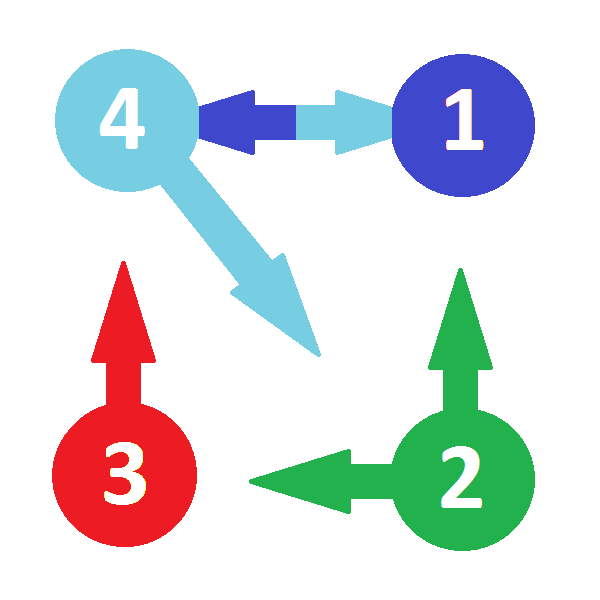
\includegraphics[scale=0.4]{imagens/grafo}
	\caption{Grafo usado nas simulações.}
	\label{grafoSimu}
\end{figure}

\noindent Além disso, todas as simulações foram realizadas com base na seguinte condição inicial:

\begin{equation}\label{x0}
x_0 = \begin{pmatrix}
0\\ 0\\ 0\\ 1
\end{pmatrix}.
\end{equation}

%%%%%%%%%%%%%%%%%%%%%%%%%%%%%%%%%%%%%%%%%%%%%
\section{Simulação do \textit{Power Method}}%
%%%%%%%%%%%%%%%%%%%%%%%%%%%%%%%%%%%%%%%%%%%%%

Na simulação do modelo mais simples do cálculo do \textit{PageRank}, o \textit{Power Method}, observa-se uma rápida convergência para cada um dos valores do vetor de estados. Isso ocorre devido a dimensão do problema usado na simulação. As cores das linhas dos gráficos, que representam os resultados das simulações, seguem o mesmo esquema das cores do grafo na figura \ref{grafoSimu}. Desta forma, as linhas do gráfico estão associadas às páginas da seguinte forma: 

\begin{itemize}
\item página 1: azul escuro,
\item página 2: verde,
\item página 3: vermelho,
\item página 4: azul claro.
\end{itemize}

\
\begin{figure}[!htb]
	\centering
	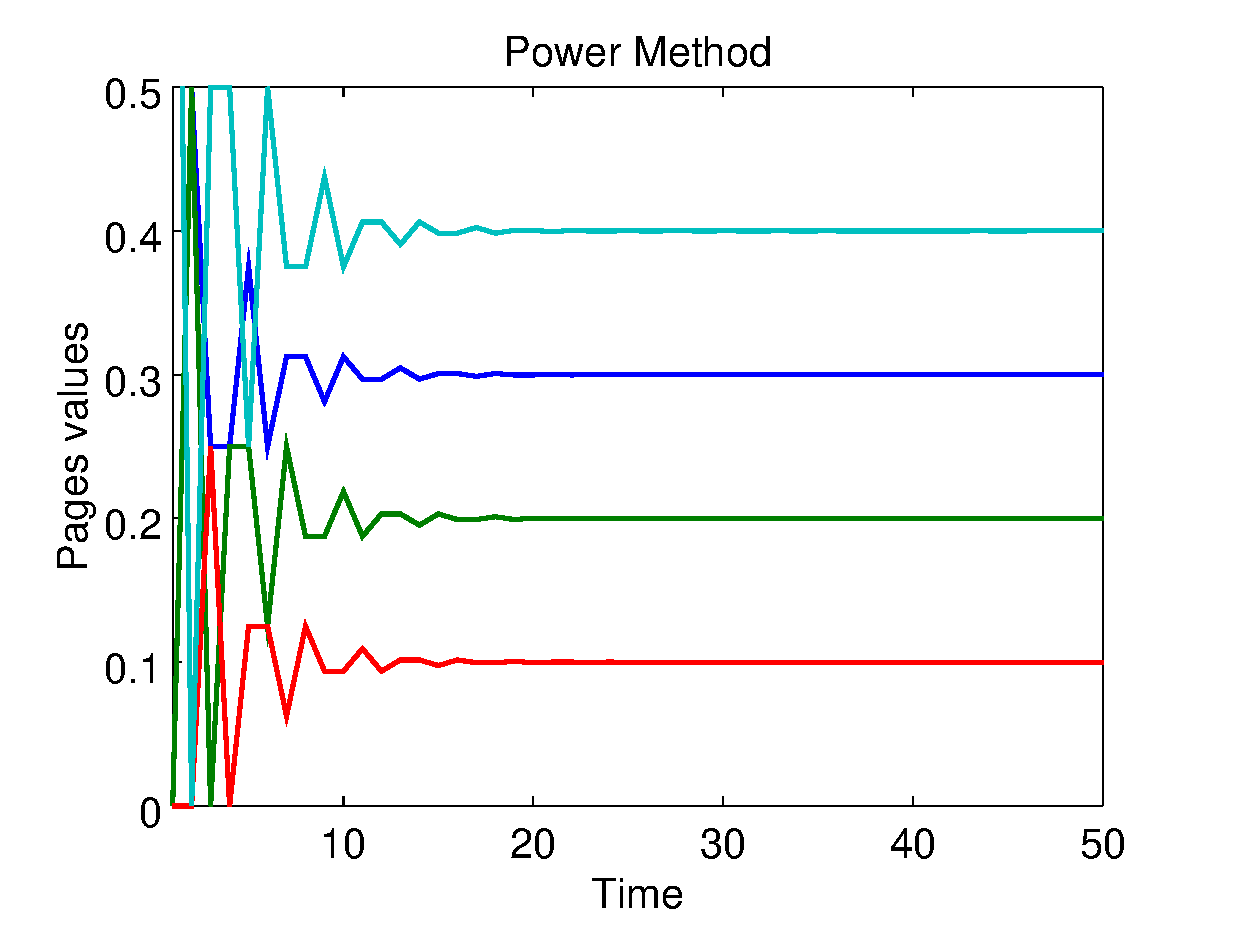
\includegraphics[scale=0.4]{imagens/powermethod}
	\caption{Resultado das simulações do \textit{Power Method}.}
	\label{powermethod}
\end{figure}

Assim pode-se observar que a página de número $4$ foi a que recebeu um maior \textit{PageRank}, dentro deste conjunto de páginas. Ao mesmo que $4$ é a página que está associada a um maior número de links, tanto de entrada quanto de saída, o que define seu alto valor de \textit{PageRank}.

Entretanto, um resultado em primeira vista parece não ser conveniente ao grafo. Ao analisar-se o valor final de $1$ observa-se que ele está na frente da página $2$, e $2$ possui mais \textit{links} de saída que $1$. Fazendo-se uma análise mais cuidadosa nota-se que $1$ possui \textit{links} de entrada e saída para $4$, ou seja por estar ligada a $4$ e por $4$ possuir alto \textit{PageRank}, o número de acessos a $1$ foi maior por estar próximo a uma página supostamente importante.     

%%%%%%%%%%%%%%%%%%%%%%%%%%%%%%%%%%%%%%%%%%%%%%%%%%%%
\section{Simulação do \textit{Teleportation Model}}%
%%%%%%%%%%%%%%%%%%%%%%%%%%%%%%%%%%%%%%%%%%%%%%%%%%%%

Na simulação do \textit{Teleportation Model}, figura \ref{teleportation}, também observa-se uma rápida convergência como nos resultados da simulação do \textit{Power Method}.

\
\begin{figure}[!htb]
	\centering
	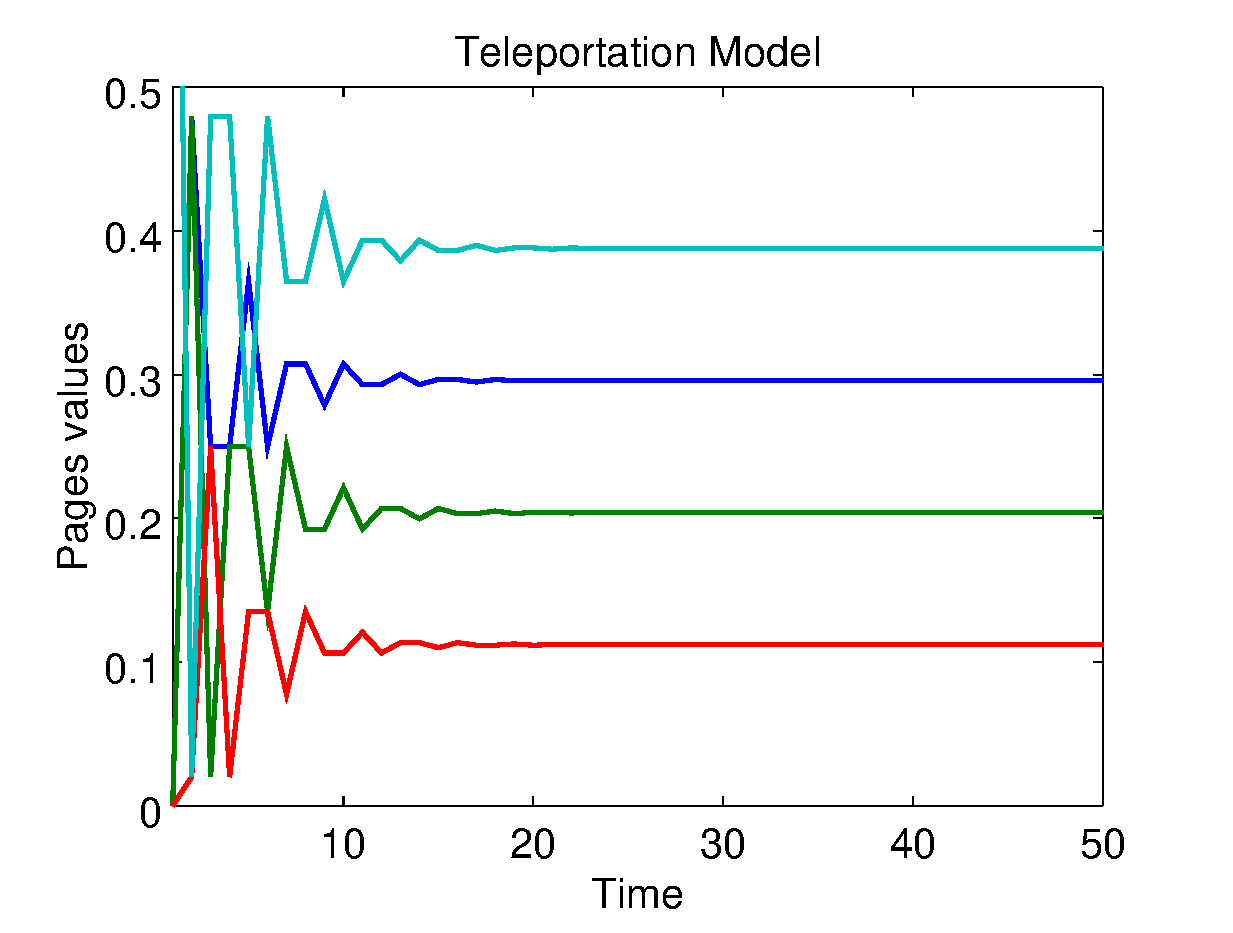
\includegraphics[scale=0.4]{imagens/teleportation}
	\caption{Resultado das simulações do \textit{Teleportation Model}.}
	\label{teleportation}
\end{figure}

Além disso uma grande semelhança é observada entre as duas simulações, como pode-se constatar na figura \ref{powertele}. Tanto a semelhança quanto a rápida convergência se devem ao fato do exemplo simulado não possuir um enorme número de estados $n$ e por ser bem comportado.

\
\begin{figure}[!htb]
	\centering
	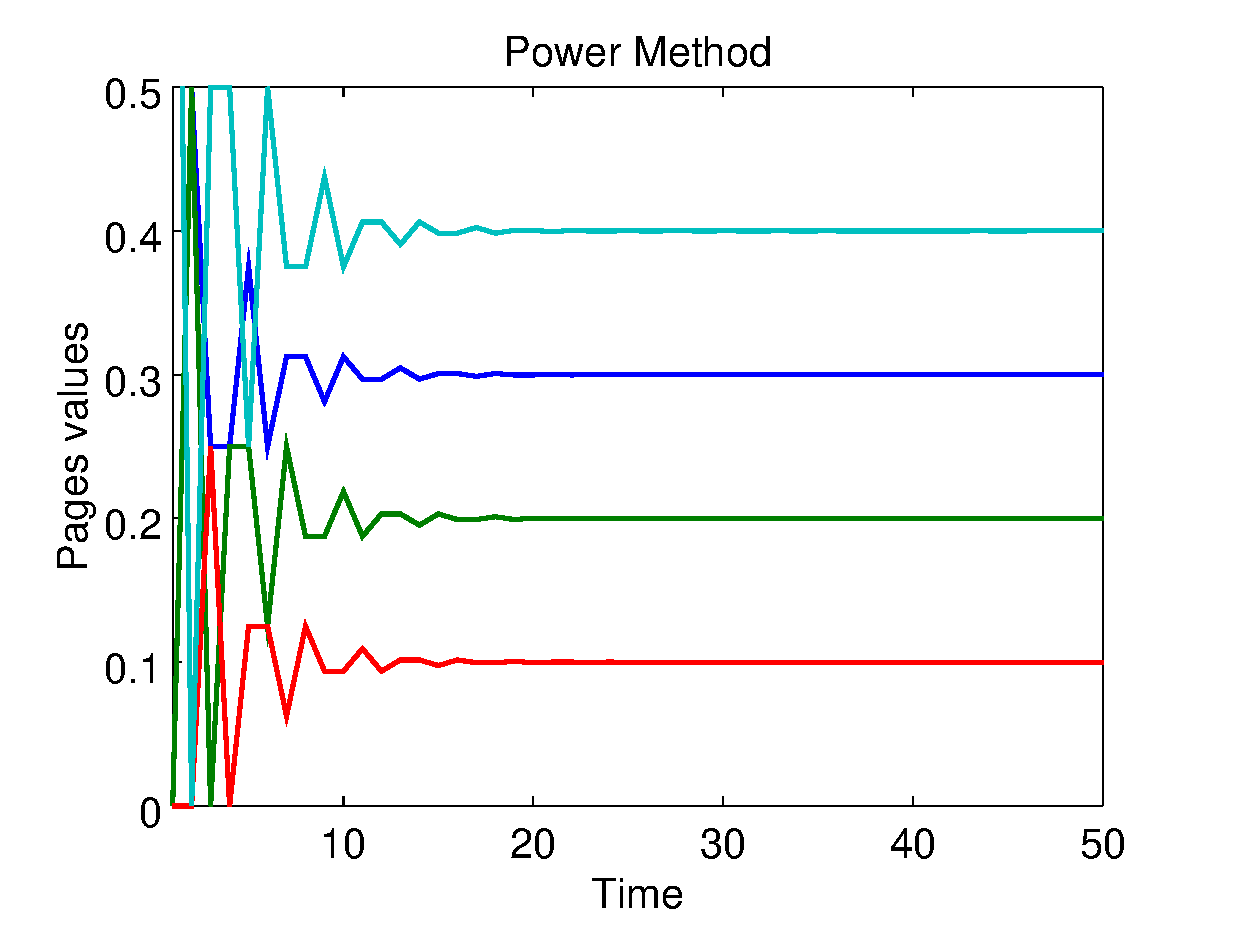
\includegraphics[scale=0.35]{imagens/powermethod}
	\hspace{0.1cm}
	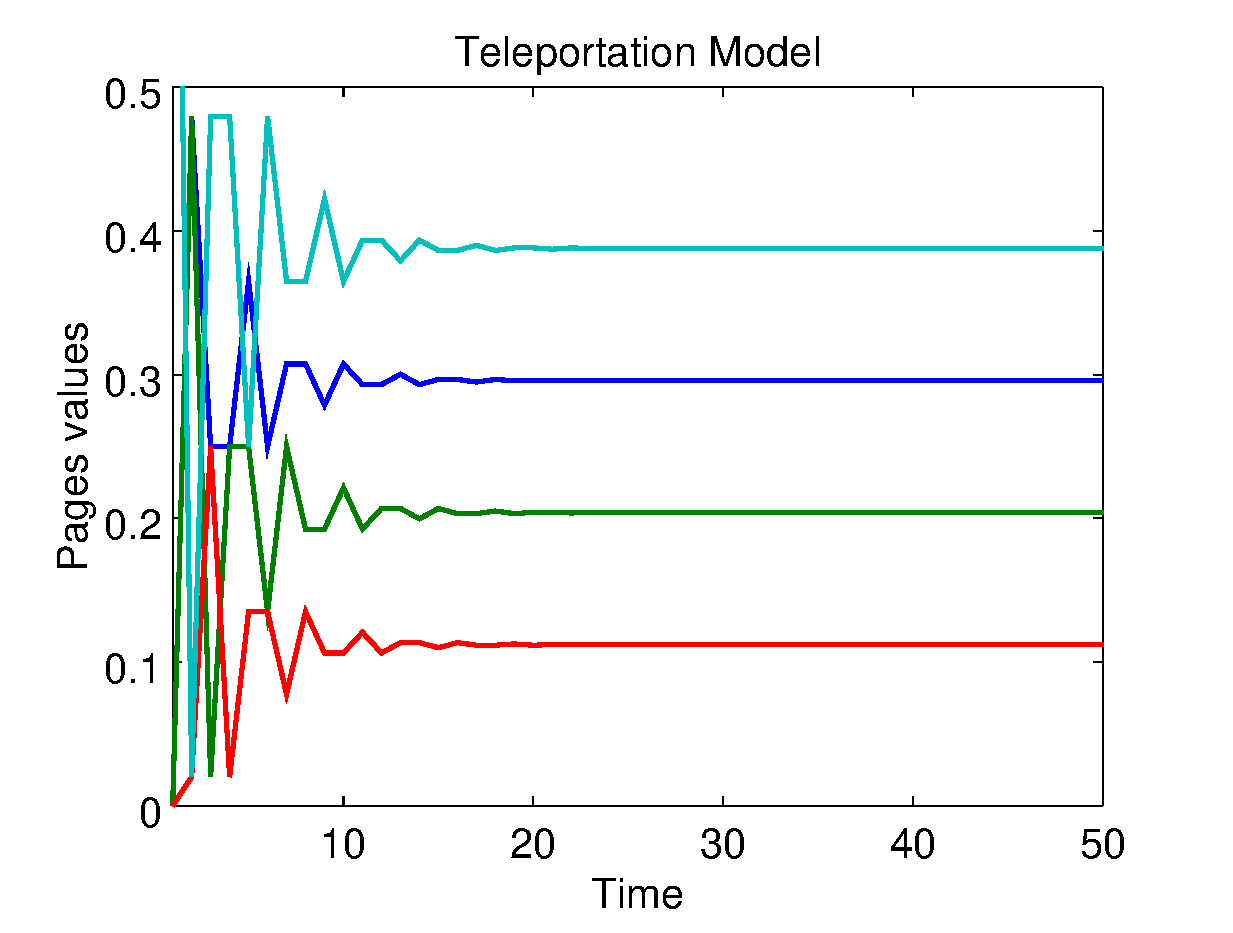
\includegraphics[scale=0.35]{imagens/teleportation}
	\caption{Comparação entre o \textit{Power Method} e o \textit{Teleportation Model}.}
	\label{powertele}
\end{figure}

%%%%%%%%%%%%%%%%%%%%%%%%%%%%%%%%%%%%%%%%%%%
\section{Simulações do Modelo Distribuído}%
%%%%%%%%%%%%%%%%%%%%%%%%%%%%%%%%%%%%%%%%%%%

As simulações do modelo distribuído foram divididas em duas subseções, uma com os resultados do modelo distribuído sem a média no tempo e outra com a média no tempo em sua forma recursiva. É possível observar que os resultados convergem com a média e não convergem sem ela.


%%%%%%%%%%%%%%%%%%%%%%%%%%%%%%%%%%%%%%%%%%%%%%%%%%%%%%%%%%%%%%%%%%%
\subsection{Simulação do \textit{Teleportation Model} Distribuído}%
%%%%%%%%%%%%%%%%%%%%%%%%%%%%%%%%%%%%%%%%%%%%%%%%%%%%%%%%%%%%%%%%%%%

No modelo distribuído sem a média no tempo observa-se uma oscilação dos estados sem que os valores das variáveis aleatórias atinjam a distribuição limite, ou seja, neste modelo sem a média no tempo não foi possível encontrar um valor de \textit{PageRank} mesmo depois de $500$ iterações. Os resultados dessa simulação estão apresentados na figura \ref{teledistributed}.

\
\begin{figure}[!htb]
	\centering
	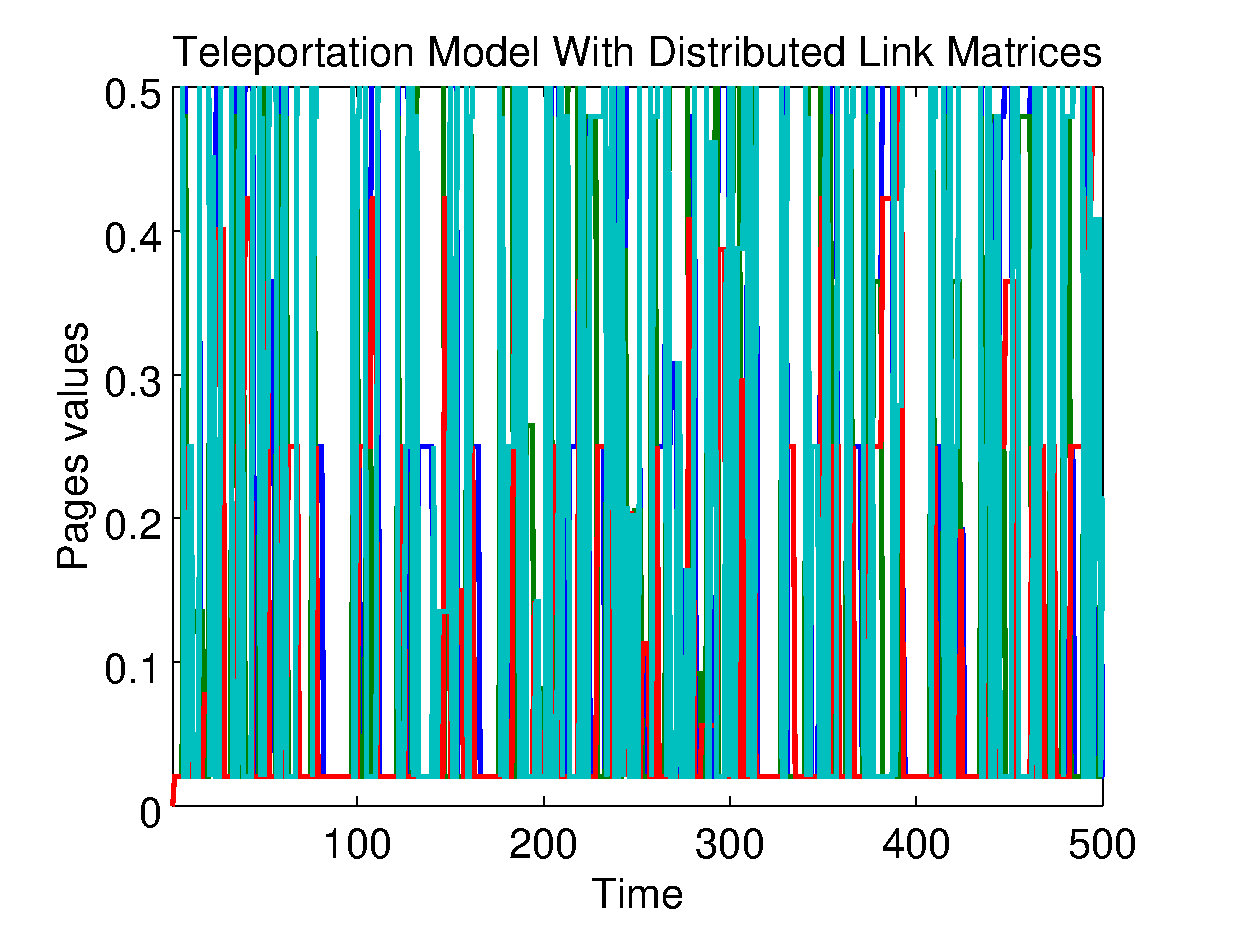
\includegraphics[scale=0.4]{imagens/teledistributed}
	\caption{Resultado das simulações do modelo distribuído.}
	\label{teledistributed}
\end{figure}

A não convergência ocorre devido as matrizes distribuídas possuirem 1's em suas diagonais, o que implicaria, por exemplo, usando-se a matriz $A_1$ como referência, nos nós $2$, $3$ e $4$ só terem saídas para si mesmo, seguindo o esquema apresentado na figura \ref{loop}.

\
\begin{figure}[!htb]
	\centering
	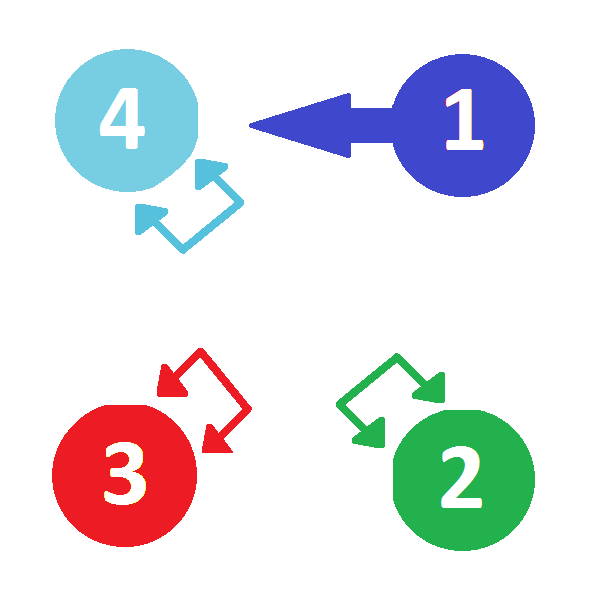
\includegraphics[scale=0.4]{imagens/loop}
	\caption{Abstração dos \textit{links} das páginas 2, 3 e 4 a partir da matriz $A_1$.}
	\label{loop}
\end{figure}

%%%%%%%%%%%%%%%%%%%%%%%%%%%%%%%%%%%%%%%%%%%%%%%%%%%%%%%%%%%%%%%%%%%%%%%%%%%%%%%%%%%%%%%%%%%%%
\subsection{O Modelo Recursivo da Média no Tempo Aplicada a Simulação do Modelo Distribuído}%
%%%%%%%%%%%%%%%%%%%%%%%%%%%%%%%%%%%%%%%%%%%%%%%%%%%%%%%%%%%%%%%%%%%%%%%%%%%%%%%%%%%%%%%%%%%%%

Entretanto, feita a média dos valores do modelo distribuído os resultados convergem, conforme é mostrado na figura \ref{timerecursive}. Mas ainda assim é possível observar algumas oscilações no gráfico, esta simulação também foi feita ao longo de $500$ iterações.

\
\begin{figure}[!htb]
	\centering
	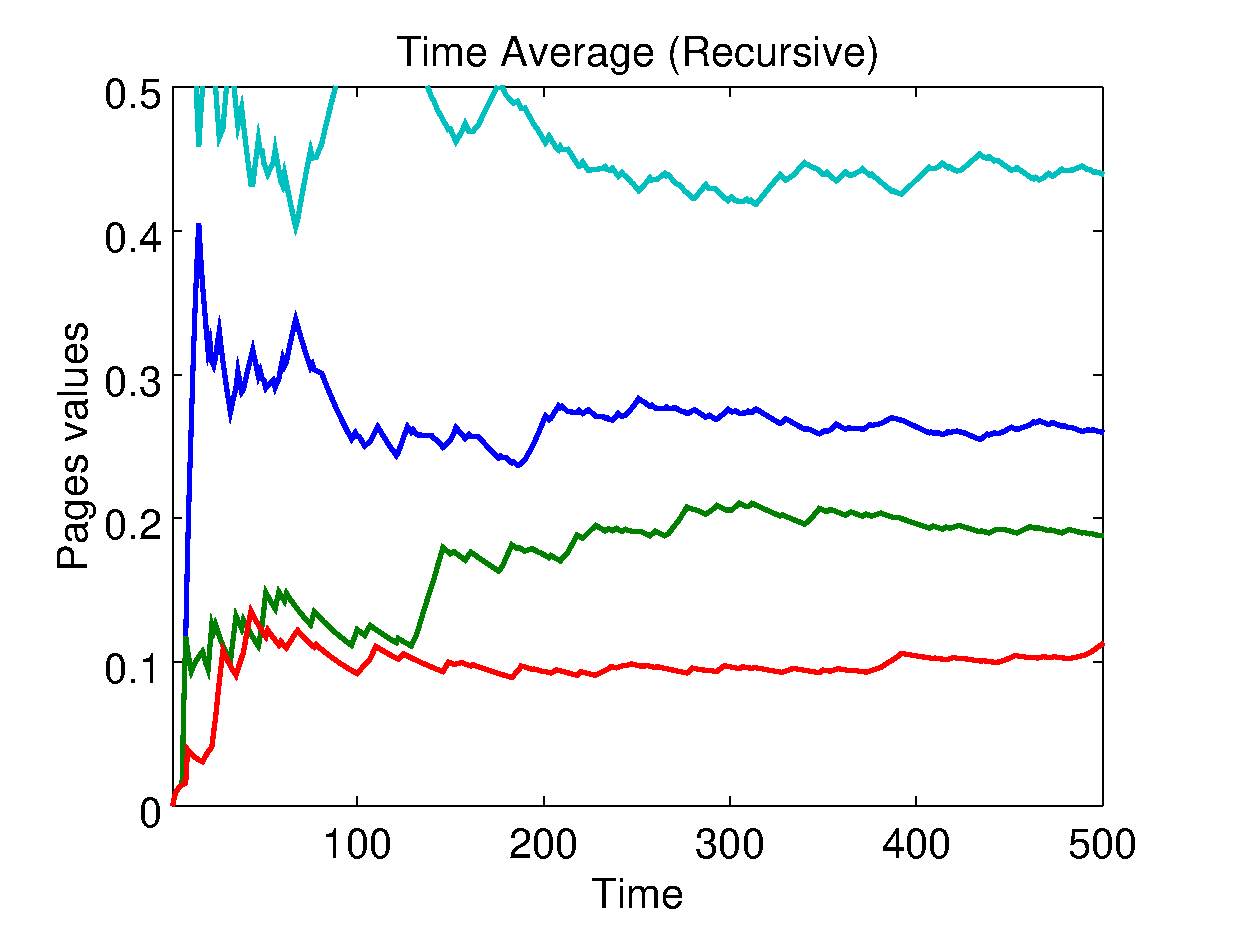
\includegraphics[scale=0.4]{imagens/timerecursive}
	\caption{Resultado das simulações do modelo distribuído com a média no tempo.}
	\label{timerecursive}
\end{figure}

Além disso, observa-se que na distribuição limite são atingidos valores bem próximos aos anteriormente encontrados para cada um dos estados no modelo do \textit{Power Method}, o que pode ser constatado a partir da figura \ref{powertime}.

\
\begin{figure}[!htb]
	\centering
	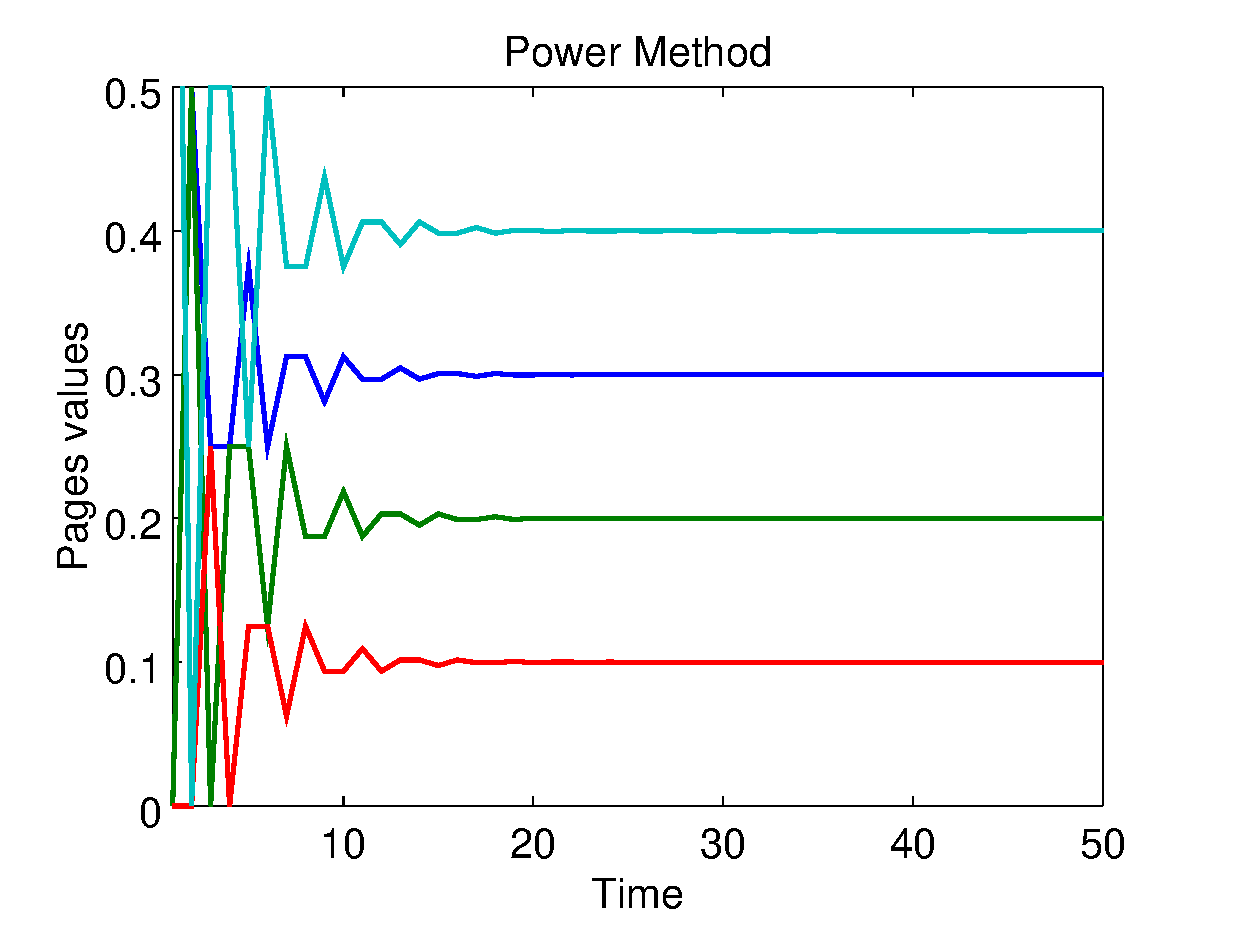
\includegraphics[scale=0.35]{imagens/powermethod}
	\hspace{0.1cm}
	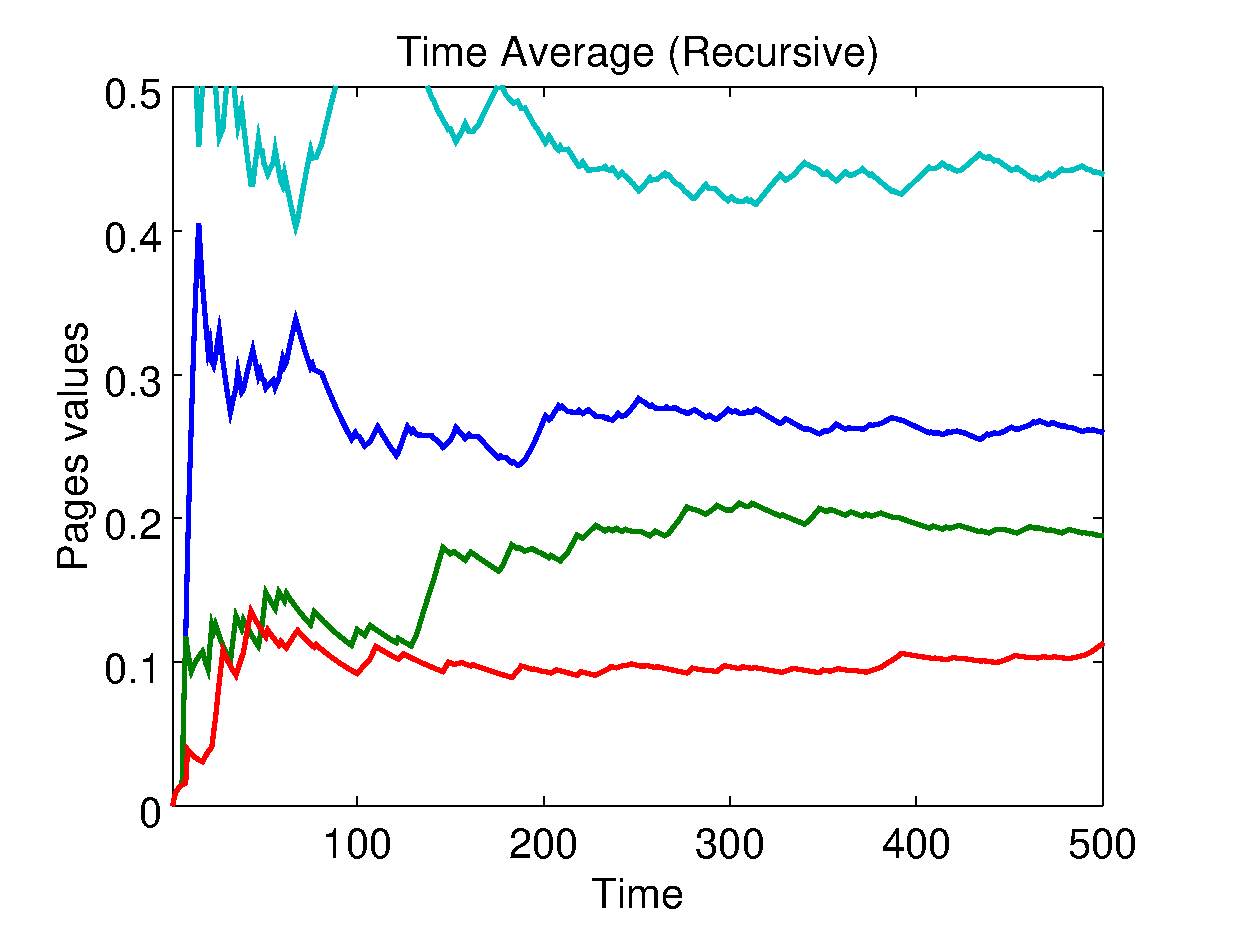
\includegraphics[scale=0.35]{imagens/timerecursive}
	\caption{Comparação entre o \textit{Power Method} e a média no tempo do modelo distribuído.}
	\label{powertime}
\end{figure}


%%%%%%%%%%%%%%%%%%%%%%%%%%%%%%%%%%%%%%%%%%%%%%%%%%%%%%%%%%%%%%%%%%%%%%%%%%%%%%%%%
\section{Método de \textit{Monte Carlo} Aplicado após Modelo Recursivo da Média}%
%%%%%%%%%%%%%%%%%%%%%%%%%%%%%%%%%%%%%%%%%%%%%%%%%%%%%%%%%%%%%%%%%%%%%%%%%%%%%%%%%

Por fim, foi feita uma simulação usando método de Monte Carlo \cite{avrachenkov2007monte}, no qual para cada uma das $500$ iterações que podem ser vistas no gráfico foram feitas mais $500$ iterações antes dos resultados serem plotados de forma a fazer uma média com os valores obtidos depois da média no tempo. Os resultados desta simulação encontram-se na figura \ref{montecarlo}.

\
\begin{figure}[!htb]
	\centering
	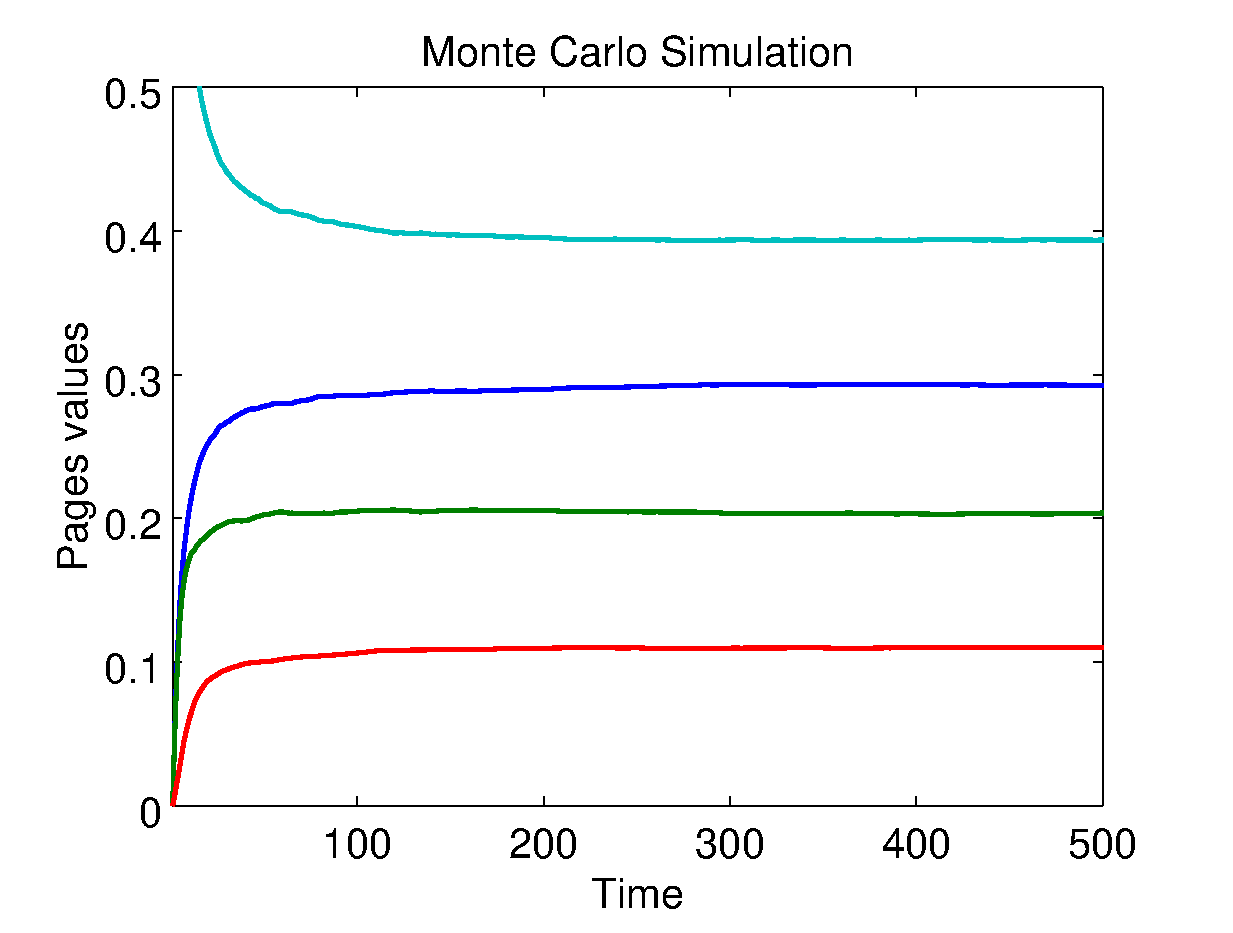
\includegraphics[scale=0.4]{imagens/montecarlo}
	\caption{Resultado das simulações com o método de Monte Carlo.}
	\label{montecarlo}
\end{figure}

Comparando a simulação em que usou-se do método de Monte Carlo com a simulação da média no tempo, observa-se que o gráfico do método de Monte Carlo possui uma curva mais suavizada, o que pode ser constatado nos resultados apresentados na figura \ref{montecarlo}. Além disso a evolução dos valores está mais bem definida, principalmente quando comparados ao valor final da distribuição limite.

\
\begin{figure}[!htb]
	\centering
	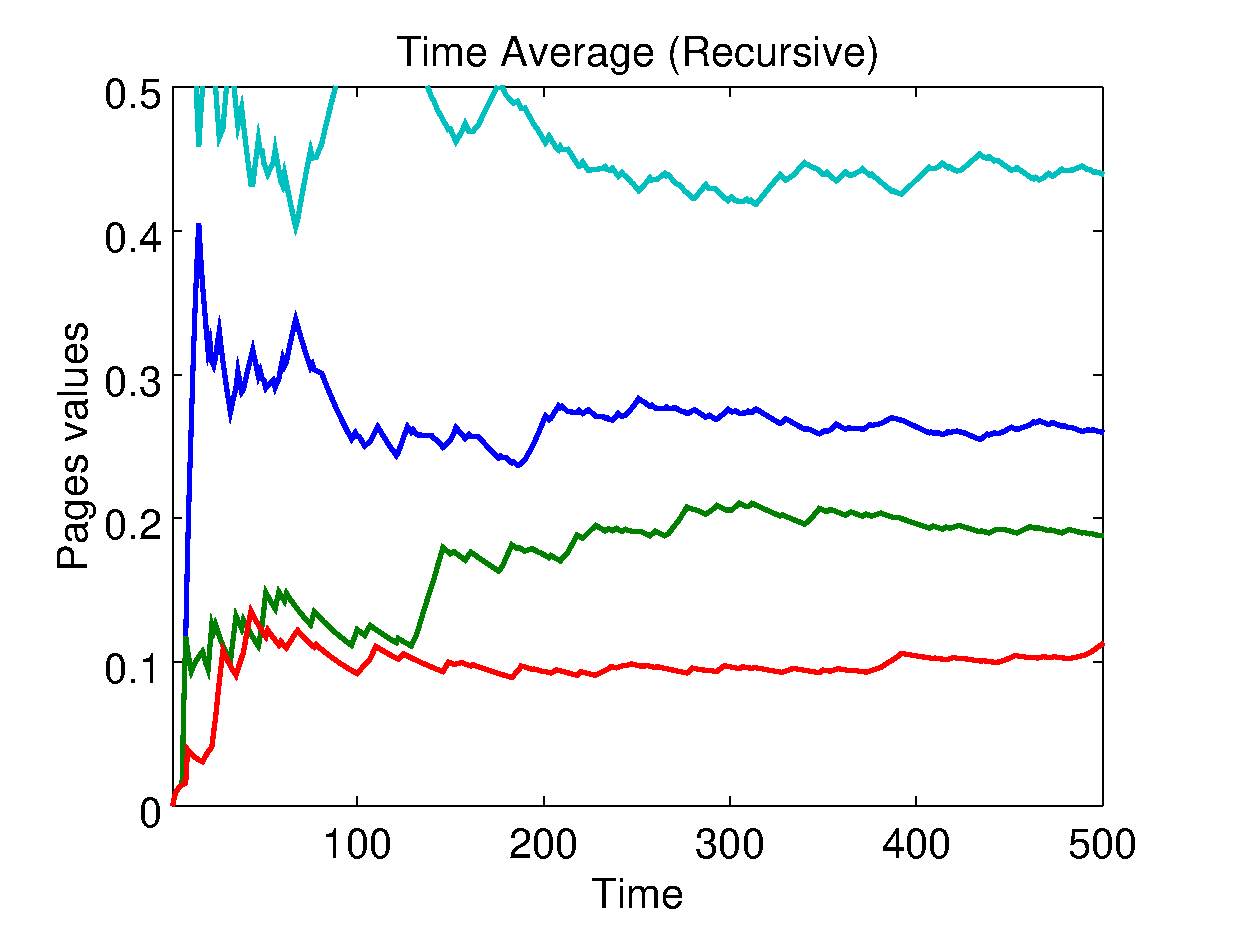
\includegraphics[scale=0.35]{imagens/timerecursive}
	\hspace{0.1cm}
	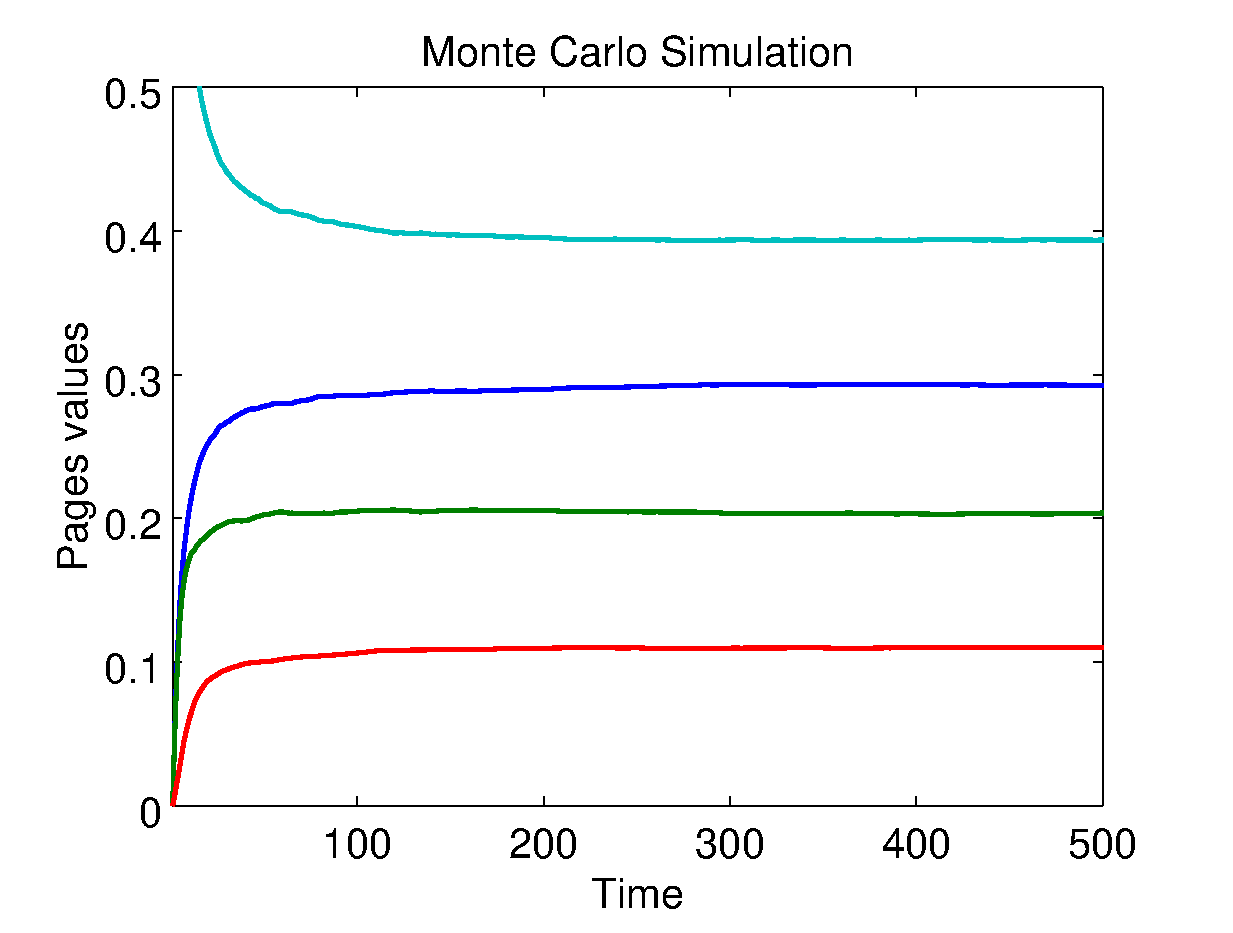
\includegraphics[scale=0.35]{imagens/montecarlo}
	\caption{Comparação entre a média no tempo do modelo distribuído e o método de Monte Carlo.}
	\label{timemonte}
\end{figure}

E ainda comparando os resultados da simulação com Monte Carlo e da simulação do \textit{Power Method} \ref{powermonte}, nota-se que os valores finais estão de acordo com os alcançados no modelo do \textit{Power Method}, o que sugere que o modelo é válido.

\
\begin{figure}[!htb]
	\centering
	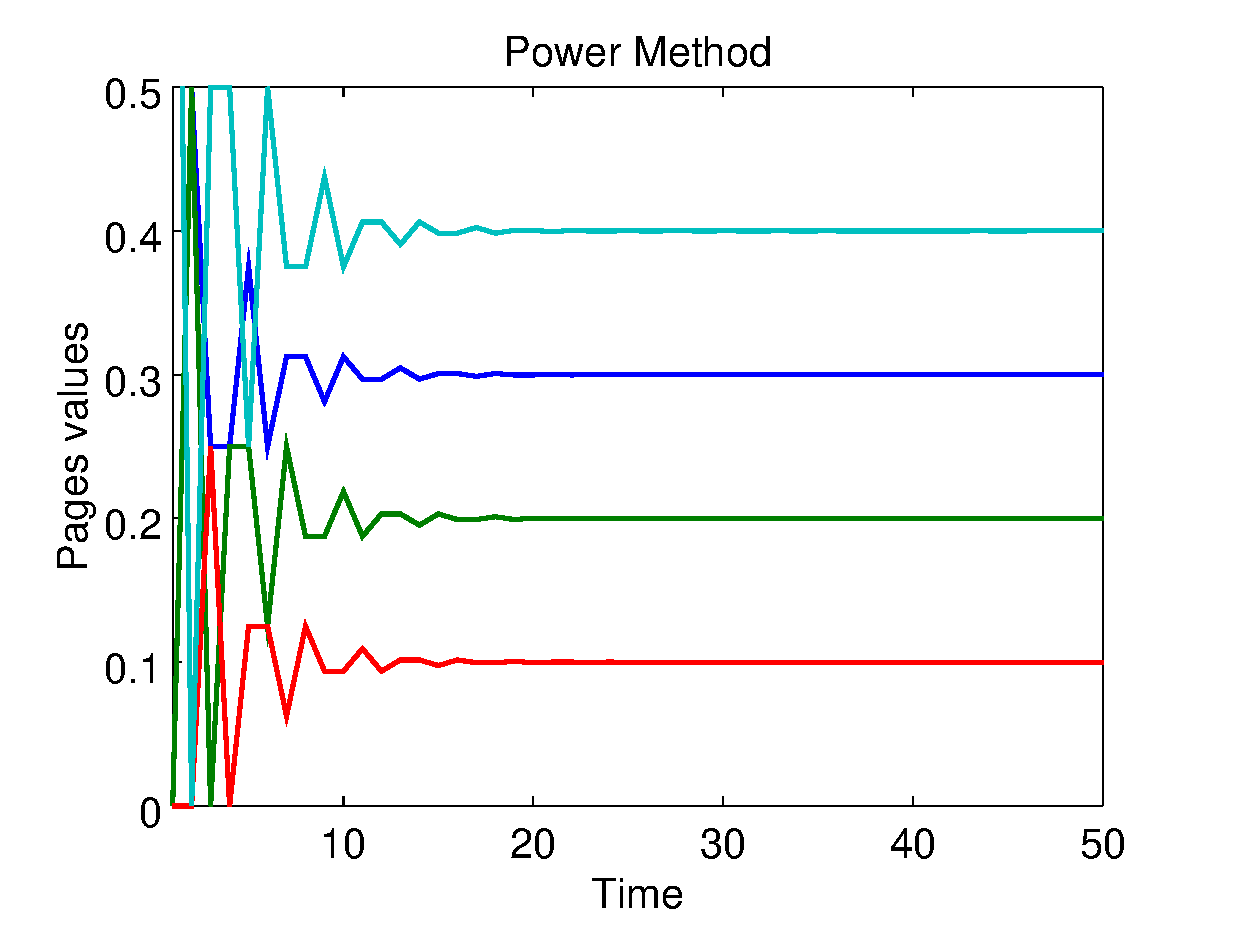
\includegraphics[scale=0.35]{imagens/powermethod}
	\hspace{0.1cm}
	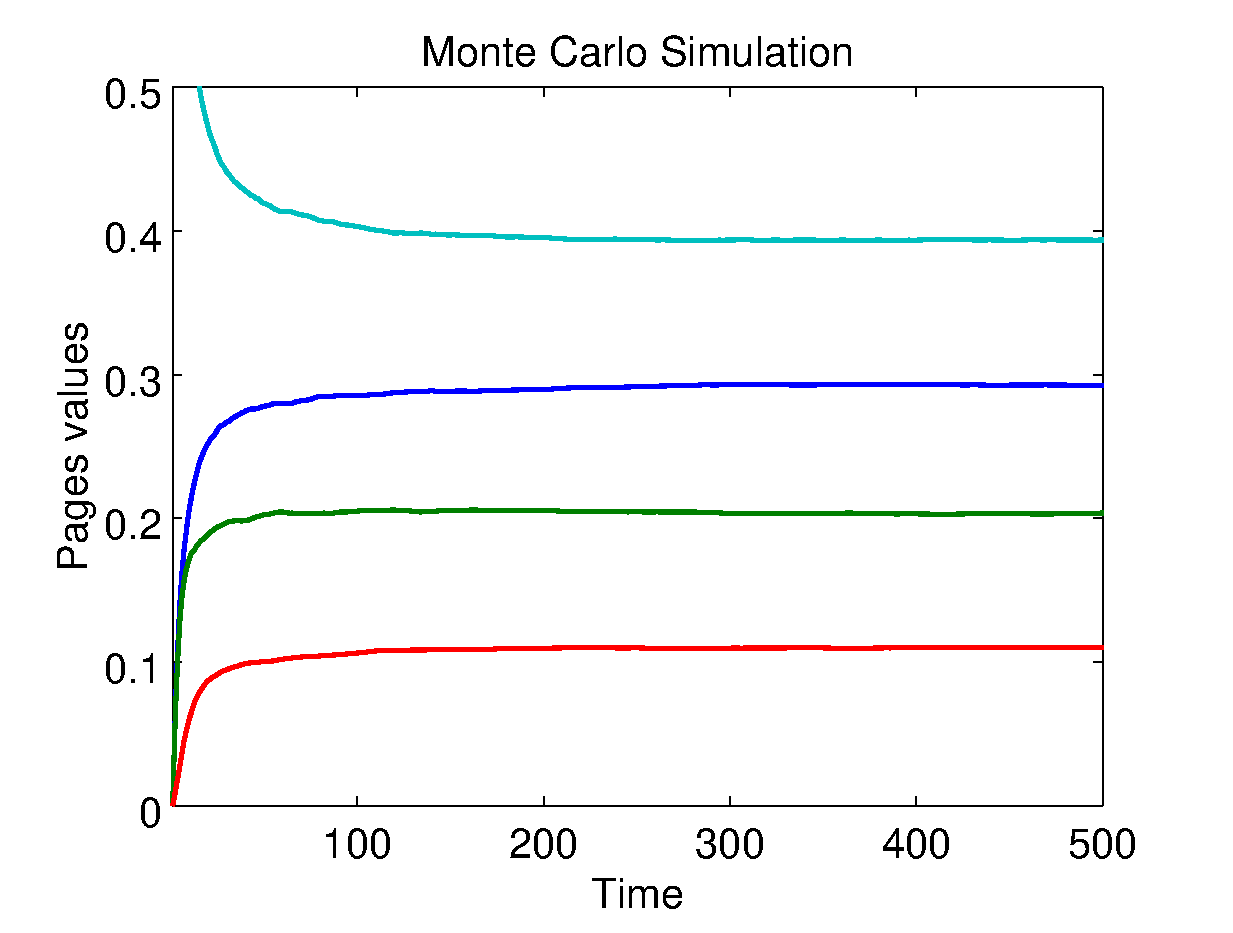
\includegraphics[scale=0.35]{imagens/montecarlo}
	\caption{Comparação entre os resultados do \textit{Power Method} e os obtidos com o método de Monte Carlo.}
	\label{powermonte}
\end{figure}